\documentclass[specialist,subf,href,colorlinks=true,14pt
%,fixint=false
,times,mtpro,specialist
]{disser}
\usepackage[
  a4paper, mag=1000, includefoot,
  left=3cm, right=1.5cm, top=2cm, bottom=2cm, headsep=1cm, footskip=1cm
]{geometry}
\usepackage[T2A]{fontenc}
\usepackage[utf8]{inputenc}
\usepackage[english,russian]{babel}
\usepackage{graphicx}
\ifpdf\usepackage{epstopdf}\fi
%\sloppy

%\usepackage{cite,enumerate,float}

\usepackage{vmargin}
\usepackage{indentfirst}
\usepackage[T2A]{fontenc}
\usepackage{graphics}
\usepackage{amsthm}
\usepackage{amsbsy}
\usepackage{amsmath}
\usepackage{amssymb}
\usepackage{amsfonts}
\usepackage{mathtext}
\usepackage{hhline}
\usepackage{longtable}
%\usepackage{fancybox,fancyhdr} 
%\usepackage{setspace}
\setcounter{tocdepth}{2}


\begin{document}
\renewcommand{\figurename}{Рисунок}
\newcommand{\class}{\textcolor[rgb]{0.5,0,0.5}}
\newcommand{\type}{\textcolor[rgb]{0.5,0.5,0}}
\newcommand{\field}{\textcolor[rgb]{0.5,0,0}}

\begin{titlepage}
	\begin{center}
		\textsc{ 
		\small{
			Московский Государственный Университет им. М.\,В.~Ломоносова \\\vspace{5pt}
 			Механико-математический факультет \\ \vspace{5pt} 
 			Кафедра вычислительной математики
 			}
 		} 
		\\\vspace{2em} 
		\textsc{\textbf{\large{Курсовая работа}}\\ \vspace{15pt}
			Студентки 410 группы\linebreak
			Нагорных Яны Валерьевны \linebreak \\ 
			\large{
				\textbf{<<Реализация библиотеки параллельной записи больших файлов с вещественными числами в текстовом представлении>>} \\\vspace{10pt} 	
				\textbf{<<Implementation of a parallel record library of large files with floating-point numbers in a text representation>>}
			} 
		}
	\end{center}
	\vspace{3em} 
	\newbox{\lbox} 
	\newlength{\maxl} \setlength{\maxl}{\wd\lbox} \hfill\parbox{15em}
	{
		\hspace*{7em}\hspace*{-7em}
		\textbf{Выполнила}\\
	 	\hfill\hbox to\maxl{\,\,Я.\,В.~Нагорных} \\ 
	}
	
	\newbox{\lbox} \hfill\parbox{15em}
	{
		\hspace*{7em}\hspace*{-7em}
		\textbf{Научный руководитель}\\
		\hfill\hbox to\maxl{\,\,д.\,ф.-м.\,н.,\, доцент К.\,Ю.~Богачев}
	}
	\\ \vspace{14pt}
	\begin{center} 
		Москва \\ 
		2018
	\end{center} 
\end{titlepage}

\tableofcontents
%\newpage
\section*{Введение}
\addcontentsline{toc}{section}{Введение}
\paragraph{Постановка проблемы.}
Печать большив массивов чисел без округления с большой точностью всегда занимает много времени.
Однако, не вся печать упирается в возможности диска, как это может показаться.
Кроме того, у печати данных мало ресурсов для ускорения.

Печать чисел с плавающей точкой также является проблемой, так как само значение числа и его экспоненту нельзя обрабатывать независимо. 

Стандартный подход недостаточно точен и в некоторых случаях дает неверные результаты. 
Кроме того использование функций стандартных библиотек \texttt{printf} и  \texttt{sprintf} достаточно затратно по времени.

\textbf{Цели работы:}
\begin{enumerate}
\item Ускорить печать больших массивов без потери точности;
\item Использовать быстрые алгоритмы печати целых чисел и чисел с плавающей точкой.
\end{enumerate}

\paragraph{Обзор предыдущих решений.} ????
\paragraph{Возможные варианты улучшений.}
Мы уже обратили внимание на то, что стандартная функция преобразования буфера в строковый тип \texttt{sprintf (char *, const char *, \dots)} работает крайне долго. 
Возникает идея применения более быстрых алгоритмов преобразования чисел в строки. 
Так например быстрое логарифмирование, разбиение числа на цифры, может заметно ускорить процесс.

Можно уменьшить число обращений к диску.
Как известно, данные, отправленные на запись, накапливаются в памяти и записываются тогда, когда получен символ переноса строки или что-то в этом роде.
Значит, можно отправлять не по одному числу на печать, а сразу готовым буффером.

Другой идеей для улучшения является использование многопоточного программирования. 
Из-за того что печать в файл должна быть строго последовательной, кажется, что ресурсов для распараллеливания немного.
Нельзя разбить исходный массив на равные части и параллельно начать печать.
Однако, так как большая часть времени уходит на преобразование чисел в строки, то можно распараллелить именно ее.
Непосредственно запись в сам файл упирается в возможности диска. 
Ее ускорить нельзя.

Также можно задуматься над улучшениями и оптимизировать сам алгоритм, несколько модифицировав вид выходного массива.
За счет этого можно уменьшить размер полученного файла.
Если будет встречаться подряд несколько одинаковых чисел, то можно не записывать в файл их все.
Также, немного уменьшит размер файла отбрасывание ненужных нулей в конце записи числа после точки.


%\newpage
\section{Описание алгоритма} \label{sec1}
Схематично работа алгоритма параллельной записи показана на Рисунке \ref{draw}.
\begin{figure}[h!]
\begin{footnotesize}
\def\svgwidth{430pt}
  \input{pics/drawing.pdf_tex}
  \caption{Работа потоков.} \label{draw}
\end{footnotesize}\end{figure}

\subsection{Используемые структуры и классы}
\paragraph{Структура \texttt{\class{reduce\_chunk}}.}
В ней находится строковый буфер, готовый для печати, и его порядковый номер \texttt{\field{chunk\_id}}.
Кроме того, хранится флаг, является ли этот \texttt{\class{reduce\_chunk}} последним.
\paragraph{Структура \texttt{\class{map\_chunk}}.}
Этот тип состоит из лямбда-функции, которая должна обработать определенный фрагмент массива чисел, и элемента типа \texttt{\class{reduce\_chunk}}, возвращаемый функцией.
\paragraph{Класс \texttt{\class{task}}.}

\paragraph{Класс \texttt{\class{mutex\_wait\_queue}}.}
Это упрощенная реализация \textit{очереди сообщений}.  
Под ней понимается очередь со следующим свойством: когда поток пытается прочитать что-то из пустой очереди, то он блокируется, до тех пор, пока какой-нибудь другой поток не положит в нее элемент.
У этой очереди есть следующие методы:
\begin{itemize}
\item \texttt{dequeue} -- достает верхний элемент из очереди, если очередь непустая.
Иначе, поток, вызвавший этот метод блокируется. Также можно передать время блокировки, по истечении которого, поток разблокируется и вернется ни с чем;
\item \texttt{dequeue\_all} -- аналогично \texttt{dequeue}, но достает все элементы, находящиеся в очереди, и складывает в переданный указатель вектор из них;
\item \texttt{enqueue} -- кладет элемент в конец очереди.
\end{itemize}
\paragraph{Класс \texttt{\class{worker\_thread}}.}
Это главный поток.
Он хранит две очереди сообщений \texttt{\field{m\_map\_queue}} и \texttt{\field{m\_reduce\_queue}}, состоящие из \texttt{\class{map\_chunk}} и \texttt{\class{reduce\_chunk}} соответственно. 
Зачем нужны такие очереди, будет сказано позже.

\subsection{Распределение задач}
Управляющий, или главный, поток \texttt{\class{worker\_thread}} вызывает функцию \texttt{create\_mappers()}, которая создает несколько потоков-обработчиков, и функцию \texttt{create\_reducer()}, которая создает печатающий поток.
Сам управляющий поток будет складывать элементы типа \texttt{\class{map\_chunk}} в очередь \texttt{\field{m\_map\_queue}}.
Потоки-обработчики будут доставать из этой очереди \texttt{\class{map\_chunk}}-и на обработку и конвертировать числа в буферы типа \texttt{\class{reduce\_chunk}}, готовые для печати.
Эти готовые буферы они будут складывать в другую очередь \texttt{\field{m\_reduce\_queue}}.
Печатающий поток должен забирать все готовые буферы из этой очереди и записывать их в правильном порядке в файл.

Что касается памяти
\subsection{Преобразование чисел в строковый тип}
Мы уже говорили о том, что вместо стандартных функций \texttt{sprintf, strtod} и подобных им, будем использовать более быстрый алгоритм преобразования чисел, а именно алгоритм \textsf{Grisu2}.

Но прежде чем приступить к самому описанию этого алгоритма, сначала приведем используемые обозначения и кратко опишем его <<предшественника>> \textsf{Grisu}.  

\subsubsection{Используемые обозначения.}
Приведем используемые далее обозначения и понятия.

Мы рассматриваем стандарт \textsf{IEEE 754} -- формат представления чисел с плавающей точкой.
Знак числа хранится отдельно, поэтому далее мы будем рассматривать положительные числа, имея ввиду, что у отрицательных чисел <<->> записан в отдельном бите.

Вообще, число $v$ с плавающей точкой по основанию $b$ представляется в памяти как $$v = f_v \times b^{e_v},$$ где основание $b$ в стандарте \textsf{IEEE 754} равно $2$. $f_v$ -- целое значение или \textit{мантисса}, а $e_v$ -- \textit{показатель}.

Любая мантисса $f$ может быть представлена как $$f = \sum\limits_{i=0}^{p-1} d_i \times b^i,$$ где $0 \leqslant d_i < b$. 
Числа $d_i$ -- \textit{знаки числа}.

Будем называть число \textit{нормированным}, если последний знак $d_{p-1}$ отличен от нуля.
Если экспонента может принимать любые неограниченные значения, то любое ненулевое число можно так отнормировать путем сдвига знака влево при соответствующей корректировке экспоненты. 

В стандарте \textsf{IEEE 754} представлены не все вещественные числа. 
Из-за этого, числа, которые не могут быть представлены в этом стандарте, будем округлять.
Как известно, числа с цифрой $5$ на конце, могут округляться по-разному.
Используем следующие обозначения:
\begin{itemize}
\item $[x]^\uparrow$ -- округление вверх;
\item $[x]^\Box$ -- округление до ближайшего четного: например, число \\$0.5$ округляется до $0$, а число $1.5$ до $2$;
\item $[x]^\star$ -- используется, когда неважно, как именно округлять;
\item $\tilde x = \left[ x \right]_p^s$ -- округленное число до $p$ знаков после запятой,\\ а $s$ -- один из вышеизложенных способов округления.
\end{itemize}

Количественно определим ошибку $|\tilde x - x|$ следующим образом.
Представим $\tilde x$ в виде $\tilde x=f \times b^e$, а $f$ округлим до ближайшего такого, что $|\tilde x - x| \leqslant 0.5 \times b^e$, или другими словами, до половины единицы последнего разряда \texttt{ulp} (\textit{unit in the last place}).

Для положительного числа $v=f_v \times b^{e_v}$ определим ближайшие в памяти числа к нему.
$v^{-}$ -- предыдущее число для $v$, хранящееся в памяти.
Аналогично $v^{+}$ -- следующее число за $v$.
Если $v$ наименьшее, то $v^{-} = 0$.
Если $v$ наибольшее, то $v^{+} = v + (v - v^{-})$.

Введем понятие \textit{границы} между двумя соседними числами.\\
По определению это средние арифметические $$m^- = \cfrac{v^- + v}{2} \quad \mbox{и} \quad m^+ = \cfrac{v + v^+}{2}.$$
Очевидно, что границы нельзя представить в виде чисел с плавающей точкой, так как они лежат между двумя соседними числами в памяти. 
Поэтому любое число $w$, такое что $m^- < w < m^+$, будет округлено до $v$. 
Если же $w$ совпало с одной из границ будем округлять его до ближайшего четного.

Будем говорить, что представление $R$ у числа с плавающей точкой $v$ \textit{удовлетворяет требованию} с максимальной точностью без округления, если при чтении $R$ будет представлено как $v$.

Определим тип \texttt{diy\_fp} для $x$ как беззнаковое целое число $f_x$, состоящее из $q$ битов, и знакового целого числа $e_x$ неограниченного диапазона.
Значение $x$ можно вычислить как $x= f_x \times 2^{e_x}$. 
Другими словами, строим отображение:
$$x \mapsto (f_x, e_x), \qquad f_x \in \left(0, 2^{q-1}\right] \cap \mathbb{Z}, \quad e_x \in \mathbb{Z},\quad \mbox{т.ч.}\, x=f_x \times 2^{e_x}$$
Введем произведение двух таких типов.
Вычислять и обозначать его будем следующим образом:
$$x \otimes y := \left[ \frac{f_x \times f_y}{2^q}\right]^\uparrow \times 2^{e_x+e_y+q}.$$
\subsubsection{Алгоритм \textsf{Grisu}}
В статье \cite{1} описан алгоритм \textsf{Grisu} и его улучшения, также доказана точность его работы.
Опишем кратко этот алгоритм.
\paragraph{Идея алгоритма.}
Предполагается, не умаляя общности, что у числа с плавающей точкой $v$ отрицательный показатель. 
Тогда это число можно выразить как $$v=\cfrac{f_v}{2^{-e_v}}.$$
Десятичные цифры $v$ могут быть вычислены путем нахождения десятичного показателя $t$, для которого $1 \leqslant \cfrac{f_v \times 10^t}{2^{-e_v}} < 10$.

Первая цифра является целой частью этой дроби. 
Последующие цифры вычисляются путем повторного использования оставшейся дроби: нужно умножить числитель на $10$ и взять целую часть от вновь полученной дроби.

Идея \textsf{Grisu} состоит в кэшировании приблизительных значений дробей $\cfrac{10^t}{2^{e_t}}$.
Дорогостоящих операций с большими числами не будет: они заменяются операциями с целыми числами фиксированного размера.

Кэш для всевозможных значений $t$ и $e_t$ может быть весьма затратным. 
Из-за этого требования к кеш-памяти в \textsf{Grisu} упрощены: кэш хранит только нормированные приближения с плавающей точкой всех соответствующих степеней десяти, а не самих дробей. Таким образом хранятся $$\tilde{c}_k := \left[ 10^k \right]_q^{\star},$$ где $q$ -- точность кэшированных чисел.
Кэшированные числа сокращают большую часть вычисления экспоненты $v$, так что остается вычислить только показатель. 

В процессе вычисления знаков используются степени десяти с экспонентой $e_{\tilde{c_t}}$, близкой к $e_v$. 
Разница между двумя показателями будет небольшой.
Фактически, \textsf{Grisu} выбирает степени десяти так, что разница лежит в определенном диапазоне. 

\paragraph{Реализация.}
Алгоритм \textsf{Grisu}: \begin{itemize}
\item \textit{Вход:} положительное число с плавающей точкой $v$ точности $p$.
\item \textit{Условие:} точность \texttt{diy\_fp} удовлетворяет $q \geqslant p + 2$, а кеш степеней десяти состоит из предварительно вычисленных нормированных округленных  \texttt{diy\_fp} со значениями $\tilde{c}_k := \left[ 10^k \right]_q^{\star}$
\item \textit{Вывод:} строковое представление в основании 10 для $V$ такое, что $[V]^{\Box}_p = v$. 
То есть при чтении числа $V$, оно должно быть округлено до $v$.
\end{itemize}

Шаги алгоритма:
\begin{enumerate}
\item \textit{Преобразование:} определим нормированный \texttt{diy\_fp} $w$ такой, что $w = v$.
\item \textit{Кэширование степеней:} сначала вычисляем $$k = -\left\lceil \log_{10} {2^{\alpha -e+q-1}} \right\rceil,$$  а затем находим с заданной точностью $$\tilde{c}_{-k} = f_c \times 2^{e_c}$$ такое, что $\alpha \leqslant e_c + e_w + q \leqslant \gamma$. ($\alpha$ и $\gamma$ заданные заранее параметры, причем $\alpha + 3 \leqslant \gamma$. Считаем $\alpha=0$ и $\gamma=3$).
\item \textit{Произведение:} пусть $$\tilde{D} = f_D \times 2^{e_D} := w \otimes \tilde{c}_{-k}.$$
\item \textit{Выход:} определим искомое $$V := \tilde{D} \times 10^k.$$ 
Вычислим десятичное представление $\tilde{D}$, за которым следует строка \texttt{e} и десятичное представление $k$.
\end{enumerate}
Поскольку значение \texttt{diy\_fp} больше, чем значение входного числа, преобразование в шаге 1 дает точный результат. 
По определению \texttt{diy\_fp}-ы имеют бесконечный диапазон экспоненциальности, и следовательно, показатель степени $w$ достаточно велик для нормирования. 
Заметим, что показатель $e_w$ удовлетворяет $e_w \leqslant e_v - (q - p)$. 
 
Легко показать, что $\forall \, i \quad 0 < \tilde{e}_{c_i} - \tilde{e}_{c_{i-1}} \leqslant 4$, и поскольку кеш неограничен, требуемый $\tilde{c}_{-k}$ должен находиться в кэше. 
Это является причиной первоначального требования $\gamma \geqslant \alpha + 3$.
Разумеется, бесконечный кеш не нужен. 

Результатом \textsf{Grisu} является строка, содержащая десятичное представление $\tilde{D}$, за которым следуют символ \texttt{e} и $k$ знаков. 
Таким образом, он представляет собой число $V: = \tilde{D} \times 10^k$. 
Утверждается, что представление $V$ у числа $v$ \textit{удовлетворяет требованию} с точностью $p$.

\subsubsection{Алгоритм \textsf{Grisu2}}
Но у \textsf{Grisu} есть существенный недостаток.
Например, при значениях по умолчанию $\alpha = 3$ и $q=64$ получаем $k=-19$, а значит, число 1 будет напечатано в виде \texttt{10000000000000000000e-19.}
Поэтому будем использовать \textsf{Grisu2}.
Этот алгоритм является усовершенствованием предыдущего и не записывает лишние нули в конец числа.
Так, если целочисленный тип \texttt{diy\_fp} содержит более двух дополнительных битов, или так называемых флагов, то эти флаги можно использовать для сокращения длины выходной строки.
В отличие от \textsf{Grisu} алгоритм \textsf{Grisu2} не генерирует полное десятичное представление, а просто возвращает значащие цифры и соответствующий показатель. 
Затем процедура форматирования объединяет эти данные для получения представления в требуемом формате.

\paragraph{Идея алгоритма.} 
Как описано выше, \textsf{Grisu2} использует дополнительные флаги для создания более короткой выходной строчки. 
Также \textsf{Grisu2} не будет работать с точными числами, а вместо этого будет вычислять аппроксимации $m^{-}$ и $m^+$. 
Чтобы избежать ошибочных результатов, которые не удовлетворяют требованиям, добавляется так называемое безопасное пространство (\textit{safety margin}) вокруг приблизительных границ.
То есть увеличивается диапазон, в котором, согласно алгоритму, может оказаться полученное число.  
Как следствие, \textsf{Grisu2} иногда может вернуть не самое оптимальное представление: оно может лежать вне изначальных границ. 
Во избежание таких проблем добавляется третий дополнительный флаг. Итого, $q \geqslant p + 3$.

\paragraph{Реализация.}
Алгоритм \textsf{Grisu2}: \begin{itemize}
\item \textit{Вход:} положительное число с плавающей точкой $v$ точности $p$.
\item \textit{Условие:} точность \texttt{diy\_fp} удовлетворяет $q \geqslant p + 3$, а кеш степеней десяти состоит из предварительно вычисленных нормированных округленных  \texttt{diy\_fp} значений $\tilde{c_k} := \left[ 10^k \right]_q^{\star}$
\item \textit{Вывод:} десятичные знаки $d_i$, где $0 \leqslant i \leqslant n$ и целочисленное $K$, такое что $V:=d_0\dots d_n \times 10 ^K$ удовлетворяет $[V]^{\Box}_p = v$. 
\end{itemize}

Шаги алгоритма:
\begin{enumerate}
\item \textit{Границы:} вычисляем границы для $v$: $m^{-}$ и $m^{+}$. 
\item \textit{Преобразование:} определим \texttt{diy\_fp} для $w^+$ так ,что $w^+ = m^+$. 
Определим также \texttt{diy\_fp} для $w^-$ так, что $w^{-} = m^-$ и $e_w^- = e_w^+$.
\item \textit{Кэширование степеней:} находим с заданной точностью $$\tilde{c}_{-k} = f_c \times 2^{e_c}$$ такое, что $\alpha \leqslant e_c + e_w + q \leqslant \gamma$.
\item \textit{Произведение:} вычисляем \begin{align*}
&\tilde{M}^- := w^- \otimes \tilde{c}_{-k}; \\
&\tilde{M}^+ := w^+ \otimes \tilde{c}_{-k};
\end{align*}и пусть также \begin{align*} & M_\uparrow^- := \tilde{M}^- + 1 \texttt{ulp};\\
& M_\downarrow^+ := \tilde{M}^+ - 1 \texttt{ulp};\\
& \delta := M_\downarrow^+ - M_\uparrow^-.
\end{align*}
\item \textit{Количество разрядов:} находим наибольшее $\kappa$ такое,\\ что $M_\downarrow^+ \mod 10^\kappa \leqslant \delta$ и определим $P:= \left\lfloor \cfrac{M_\downarrow^+}{10^\kappa} \right\rfloor$.
\item \textit{Выход:} определим $V:= P \times 10^{k + \kappa}$. 
Получаем десятичные знаки $d_i$ и число $n$ путем вычисления десятичного представления $P$.
Положим $K:=k+\kappa$ и возвращаем его с $n$ знаками $d_i$.
\end{enumerate}

\textsf{Grisu2} не дает никаких гарантий относительно краткости длины результата. 
Его результатом является кратчайшее возможное число в интервале от $M_\uparrow^- \times 10^k$ до $M_\downarrow^+ \times 10^k$ включительно, где $M_\uparrow^- \times 10^k$ и $M_\downarrow^+ \times 10^k$  зависят от точности $q$ для \texttt{diy\_fp}.
Чем больше $q$, тем ближе $M_\uparrow^- \times 10^k$ и $M_\downarrow^+ \times 10^k$ к фактическим границам $m^-$ и $m^+$. 

Для наглядности на Рисунке \ref{pic2} приведен пример работы \textsf{Grisu2}.
В частности, видно, что алгоритм отбрасывает лишние нули в конце числа и что выбирает более короткую запись числа. 
Иррациональное число \textsf{Grisu2} напечатал с машинной точностью.
\begin{figure}[h!]
\begin{center}
\texttt{ 
\begin{tabular}{|l|c|l|}
\hhline{|-|~|-|}
  array[0] = 1;				& & 1 \\
  array[1] = 1.2;			& & 1.2 \\
  array[2] = 1.23;			& & 1.23\\
  array[3] = 1.23400000;			& & 1.234 \\
  array[4] = 1.23456789;	& & 1.23456789\\
  array[5] = -1;			& & -1\\
  array[6] = -1.234;		& $\longrightarrow$ & -1.234\\
  array[7] = sqrt (2);		& & 1.4142135623730952\\
  array[8] = 1234e-36;		& & 1.234e-33\\
  array[9] = 0.000000123;	& & 1.23e-7\\
  array[10] = 0.123;		& & 0.123\\
  array[11] = 12.3;	& & 12.3\\
  array[12] = 123.000;	& & 123\\
\hhline{|-|~|-|}
\end{tabular}
}
\textit{ 
\begin{tabular}{ccc}
$\qquad\quad$ массив $\qquad\quad$ & $\qquad\qquad$ & выходной файл \\
\end{tabular}
}
\caption{Полученный с помощью \textsf{Grisu2}, выходной файл для данного массива.} \label{pic2}
\end{center}
\end{figure}

\subsubsection{Улучшения для алгоритма}
Будем использовать следующее улучшение.
Пусть в массиве есть $n$ подряд идущих одинаковых чисел с заданной точностью, то есть $\forall i: \, 1 \leqslant i < n$ верно, что $\|x_i - x_{i-1}\| \leqslant \varepsilon$, где $\varepsilon$ -- машинная точность.
В таком случае сократим запись $n$ чисел и вернем строку вида \texttt{n*x}.
Таким образом, если в нашем массиве много повторяющихся чисел, то выходная строчка будет гораздо короче, а значит, можно ускорить программу и уменьшить размер выходного файла.
Для этого также нужно модифицировать алгоритм чтения, чтобы он мог обрабатывать запись вида \texttt{n*x}.

Запись целых чисел, означающих количество повторяющихся элементов массива, также можно ускорить.
Для этого используется алгоритм 2 из статьи \cite{2}.
Суть алгоритма заключается в быстром логарифмировании числа по основанию 10.

%\newpage
\section{Результаты работы и ускорение}
Чтобы проверить эффективность работы алгоритма параллельной записи, описанного в \ref{sec1}, проведено сравнение с алгоритмом стандартной печати: \vspace{12pt}
\begin{center}
\texttt{
\begin{tabular}{ll}
 $\quad$ & for (int i = 0; i < n;)\\
 $\quad$ & $\,\,$ \{ \\
 $\quad$ & $\,\,\quad$ for (int j = 0; j < m; j++, i++)\\
 $\quad$ & $\,\,\quad\quad$ fprintf (f, '' \%.16f'', a[i]);\\
 $\quad$ & $\,\,\quad$ fprintf (f, ''$\mathtt{\backslash n}$''); \\
 $\quad$ & $\,\,$ \} \\
\end{tabular}}\\
\end{center}
Здесь $n$ -- размер массива, а $m$ -- количество чисел, записываемых в одну строку.
Стандартная печать будет записывать числа с 16 знаками после запятой.

Для всех дальнейших тестов было сделано следующее.
Оба выходных файла, полученные работой параллельного алгоритма и стандартного, считывались вновь. 
Затем вычислялась разница между считанным числами.
Во всех запусках погрешность не превышала машинной точности, что говорит о точности работы реализованного алгоритма.

\subsection{Тест 1. Массив случайных чисел} \label{test1}
Оба алгоритма запускались на одних и тех же массивах вещественных чисел, сгенерированных случайным образом. 
Этот тест полезен тем, что в реальных моделях данные могут задаваться каким-либо распределением (например, нормальным), где все числа являются вещественными и различными.

Описанный в Разделе \ref{sec1} алгоритм параллельной записи запускался с разным числом потоков на машине с 6 ядрами.

Время работы в секундах для обоих алгоритмов приведено в Таблице 1.
Также в таблице приведен размер полученного текстового файла.
Под числом потоков понимается число потоков-обработчиков. 
Таким образом реально задействовано на два потока больше, так как помимо обработчиков есть еще управляющий поток и печатающий.
\begin{center}
\begin{longtable}{||c|c|c|c|c|c|c||}
\hline
\hline
Размер & \multicolumn{4}{c|}{Число потоков} & Стандартная & Размер\\
\hhline{~|-|-|-|-|~|~|}
массива & 6 & 4 & 2 & 1 & печать &файла\\
\hline
\hline
 & 0.593 & 0.880 & 1.620 & 3.196 & 4.256 & \\
\hhline{~|-|-|-|-|-|~|}
$10^7$   & 0.562 & 0.841 & 1.612 & 3.239 & 4.176 & 245 MB \\
\hhline{~|-|-|-|-|-|~|}
 & 0.530 & 0.802 & 1.502 & 3.052 & 4.188 &\\
\hline
&2.571& 4.044 & 7.812 & 15.37 & 22.47 & \\
\hhline{~|-|-|-|-|-|~|}
$5 \cdot 10^7$  & 2.634 & 4.273 & 8.214 & 16.30 & 21.11 &  1.2 GB\\
\hhline{~|-|-|-|-|-|~|}
 & 2.689 & 4.179 & 7.822 & 15.32 & 20.89 & \\
\hline
 & 5.219 & 8.276 & 15.67 & 32.46 & 41.71 & \\
\hhline{~|-|-|-|-|-|~|}
$10^8$  & 5.077 & 7.970 & 15.30 & 30.57 & 41.78 & 2.4 GB\\
\hhline{~|-|-|-|-|-|~|}
& 5.189 & 8.078 & 15.37 & 30.75 & 41.96 & \\
\hline
 & 41.12 & 49.15 & 75.23 & 148.91 & 200.94 & \\
\hhline{~|-|-|-|-|-|~|}
$5 \cdot 10^8$ & 40.23 & 50.08 & 75.92 & 149.08 & 200.33 & 12 GB\\
\hhline{~|-|-|-|-|-|~|}
 & 41.23 & 49.16 & 74.92 & 148.52 & 200.69 & \\
\hline
\hline
\end{longtable}
\small{Таблица 1.}
\end{center}

Также стоит заметить, что отношение времени работы при увеличении количества потоков заметно уменьшается, и при увеличении размеров массива стремится к обратному отношению числа потоков.
Наглядно зависимость времени от числа потоков для массива размером $10^8$ изображена на Рисунке \ref{pic3}.
\begin{figure}[h!]
\begin{minipage}[h]{0.5\linewidth}
\center{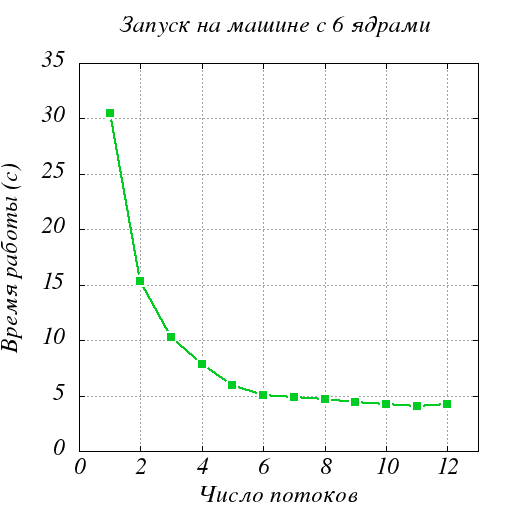
\includegraphics[width=1\linewidth]{./pics/time.png}}
\end{minipage}
\hspace{10pt}
\begin{minipage}[h]{0.5\linewidth}
\center{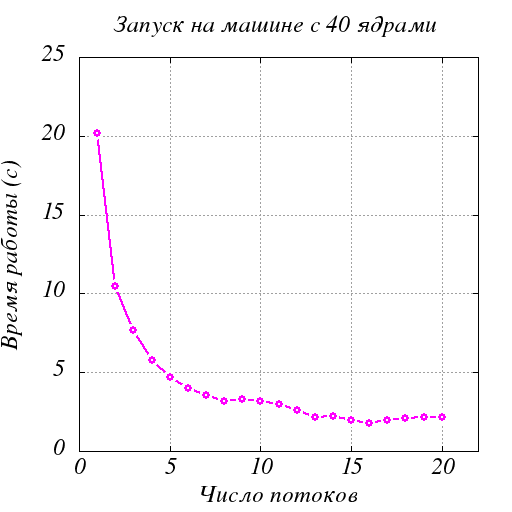
\includegraphics[width=1\linewidth]{./pics/time40.png}}
\end{minipage} 
\caption{Зависимость времени работы от числа потоков.} \label{pic3}
\end{figure}

Тот факт, что отношения работы не строго пропорциональны, объясняется несколькими фактами.
Во-первых, часть времени, хоть и небольшую при таких данных, занимала запись на диск.
Во-вторых, не все потоки могли быть все время задействованными.
Некоторые потоки могли обращаться к пустой очереди и тем самым тратить время на ожидание.

Среднее ускорение работы алгоритма по сравнению со стандартной печатью приведены в Таблице 2.
Ускорение на одном потоке демонстрирует ускорение работы \textsf{Grisu2} по сравнению со стандартной печатью.
\begin{center}
\begin{tabular}{||c|c|c|c|c||}
\hline
\hline
Размер & \multicolumn{4}{c||}{Число потоков}\\
\hhline{~|-|-|-|-|}
массива & 6 & 4 & 2 & 1 \\
\hline
$10^7$ &  7.49  & 5.00 & 2.67 & 1.33 \\
\hline
$5 \cdot 10^7$ & 8.17 & 5.16 & 2.70 & 1.37 \\
\hline
$10^8$ & 8.10 & 5.16 & 2.71 & 1.34\\
\hline
$5 \cdot 10^8$ & 4.91 & 4.06 & 2.66 & 1.35\\
\hline
\hline
\end{tabular}
\\
\vspace{14pt}
\small{Таблица 2.}
\end{center}

Заметим, что при увеличении массива до определенного размера, ускорение возрастает, а затем спадает.
Первое объясняется тем, что с увеличением объема данных, потоки простаивают меньше.
Второй факт будет рассмотрен подробнее в пункте \ref{subsec2:3}.

\subsection{Тест 2. Целые числа} \label{test2}
Массив состоит из сгенерированных случайным образом целых чисел от 0 до 1000.
С помощью этого теста, во-первых, можно проверить работу с целыми числами, а во-вторых, убедиться в том, что \textsf{Grisu2} отбрасывает ненужные нули.

\begin{center}
\begin{longtable}{||c|c|c|c|c|c|c||}
\hline
\hline
Размер & \multicolumn{4}{c|}{Число потоков} & Станд. & Размер\\
\hhline{~|-|-|-|-|~|~|}
массива & 6  & 4 & 2 & 1 & печать & файла\\
\hline
\hline
 & 0.218 & 0.322 & 0.643 & 1.297 & 5.300  &\\
\hhline{~|-|-|-|-|-|}
$10^7$ & 0.222 & 0.320 & 0.649 & 1.284 & 5.245  &56 MB / 205 MB \\
\hhline{~|-|-|-|-|-|}
 & 0.210 & 0.337 & 0.650 & 1.321 & 5.312  &\\
\hline
& 1.153 & 1.664 & 3.319 & 6.362 & 27.93  &\\
\hhline{~|-|-|-|-|-|}
$5 \cdot 10^7$& 1.125  & 1.675 & 3.334 & 6.375 & 29.46  &295 MB / 1 GB\\
\hhline{~|-|-|-|-|-|}
& 1.112  & 1.662 & 3.340 & 6.490 & 29.43  &\\
\hline
 & 2.253 &  3.374 & 6.618 & 12.61 & 55.04 & \\
\hhline{~|-|-|-|-|-|}
$10^8$ & 2.235 & 3.309 & 6.712 & 12.63 & 55.70  & 590 MB / 2 GB \\
\hhline{~|-|-|-|-|-|}
 & 2.238 & 3.248 & 6.601 & 13.66 & 56.31  &\\
\hline
 & 11.98 & 16.68 & 32.14 & 62.94 & 283.61  &\\
\hhline{~|-|-|-|-|-|}
$5 \cdot 10^8$ & 11.63 & 16.68 & 32.20 & 64.08 & 290.70  &2.9 GB / 10 GB\\
\hhline{~|-|-|-|-|-|}
 & 11.32 & 16.45 & 32.09 & 64.12 & 287.54  &\\
\hline
\hline
\end{longtable}
\small{Таблица 3.}
\end{center}

Заметим, что размер файла, полученного с помощью нового алгоритма гораздо меньше размера файла, полученного стандартной печатью, так как отброшены лишние нули.
За счет этого ускорение возросло по сравнению с Тестом \ref{test1}.

\begin{center}
\begin{tabular}{||c|c|c|c|c||}
\hline
\hline
Размер & \multicolumn{4}{c|}{Число потоков}\\
\hhline{~|-|-|-|-|}
массива & 6 & 4 & 2 & 1 \\
\hline
$10^7$  & 23.98  & 16.19 & 8.17 & 4.06 \\
\hline
$5 \cdot 10^7$ & 26.15 & 17.36& 8.69 & 4.51 \\
\hline
$10^8$ & 26.37 & 16.82 & 8.38 & 4.29 \\
\hline
$5 \cdot 10^8$ & 26.38  & 17.30 & 8.93& 4.51 \\
\hline
\hline
\end{tabular}
\\
\vspace{14pt}
\small{Таблица 4.}
\end{center}

\subsection{Тест 3. Повторяющиеся числа}
Сгенерируем массив чисел из 0 и 1.
В этом случае все последовательности одинаковых подряд идущих чисел будут сворачиваться в короткую строку вида \texttt{n*x}.

Были сделаны замеры времени аналогично предыдущим тестам.
Время работы в секундах приведено в Таблице 3.
Также приведен размер файла <<со звездами>>, полученным быстрым алгоритмом, и размер файла <<без звезд>>, полученного алгоритмом стандартной печати.
\begin{center}
\begin{longtable}{||c|c|c|c|c|c|c||}
\hline
\hline
Размер & \multicolumn{4}{c|}{Число потоков} & Станд. & Размер \\
\hhline{~|-|-|-|-|~|~|}
массива & 6 & 4 & 2 & 1 & печать  & файла\\
\hline
\hline
& 0.112 & 0.181 & 0.339 & 0.652 & 3.445  &\\
\hhline{~|-|-|-|-|-|}
$10^7$ & 0.109 & 0.159 & 0.310 & 0.604 & 3.322  & 24 MB / 187 MB \\
\hhline{~|-|-|-|-|-|}
& 0.119 & 0.168 & 0.329 & 0.661 & 3.460  &\\
\hline
& 0.521 & 0.843 & 1.630 & 2.983 & 16.91  &\\
\hhline{~|-|-|-|-|-|}
$5 \cdot 10^7$ & 0.549 & 0.841 & 1.643 & 3.067 & 17.30  & 123 MB / 936 MB\\
\hhline{~|-|-|-|-|-|}
& 0.530 & 0.833 & 1.612 & 2.875 & 16.96 & \\
\hline
& 1.178 & 1.748 & 3.343 & 6.056 & 36.19 &\\
\hhline{~|-|-|-|-|-|}
$10^8$ & 1.152 & 1.678 & 3.209 & 5.959 & 36.38  & 245 MB / 1.8 GB\\
\hhline{~|-|-|-|-|-|}
& 1.163 & 1.689 & 3.290 & 6.039 &  36.41  &\\
\hline
& 5.720 & 8.354 & 15.82 & 31.50 & 182.22 &\\
\hhline{~|-|-|-|-|-|}
$5 \cdot 10^8$ &5.714 & 8.346 & 15.71 & 31.29 & 182.00  & 1.2 GB / 9.4 GB\\
\hhline{~|-|-|-|-|-|}
& 5.816 & 8.418 & 15.92 & 31.69 & 183.52  &\\
\hline
\hline
\end{longtable}
\small{Таблица 5.}
\end{center}

Среднее ускорение приведено в Таблице 6.

\begin{center}
\begin{tabular}{||c|c|c|c|c||}
\hline
\hline
Размер & \multicolumn{4}{c|}{Число потоков}\\
\hhline{~|-|-|-|-|}
массива & 6 & 4 & 2& 1 \\
\hline
$10^7$  & 30.08 & 20.13 & 10.46 & 5.33 \\
\hline
$5 \cdot 10^7$ & 31.98 & 20.32 & 10.47 & 5.74 \\
\hline
$10^8$ & 31.20 & 21.31 & 11.07 & 6.03 \\
\hline
$5 \cdot 10^8$ & 31.75 & 21.81 & 11.54 & 5.80 \\
\hline
\hline
\end{tabular}
\\
\vspace{14pt}
\small{Таблица 6.}
\end{center}

\subsection{Тест 4. Огромные массивы} \label{subsec2:3}
Здесь, как и в первом случае, числа будут генерироваться случайным образом.
Сравнивать будем стандартную печать и алгоритм, запущенный на 12 (+2) потоках.

Помимо обычного запуска, проведем и запуск с записью не на диск, а в разделяемую память \textit{shared-memory}.
Как известно, разделяемая память является самым быстром средством обмена данными между процессами.

Ранее говорилось, что скорость диска влияет на печать, но не всегда сильно.
За счет сравнения записи на диск и в \textit{shared-memory} можно оценить, это влияние.

Далее на Рисунке \ref{grap} приведена зависимость времени работы от размера массива.
\begin{figure}[h!]
\center{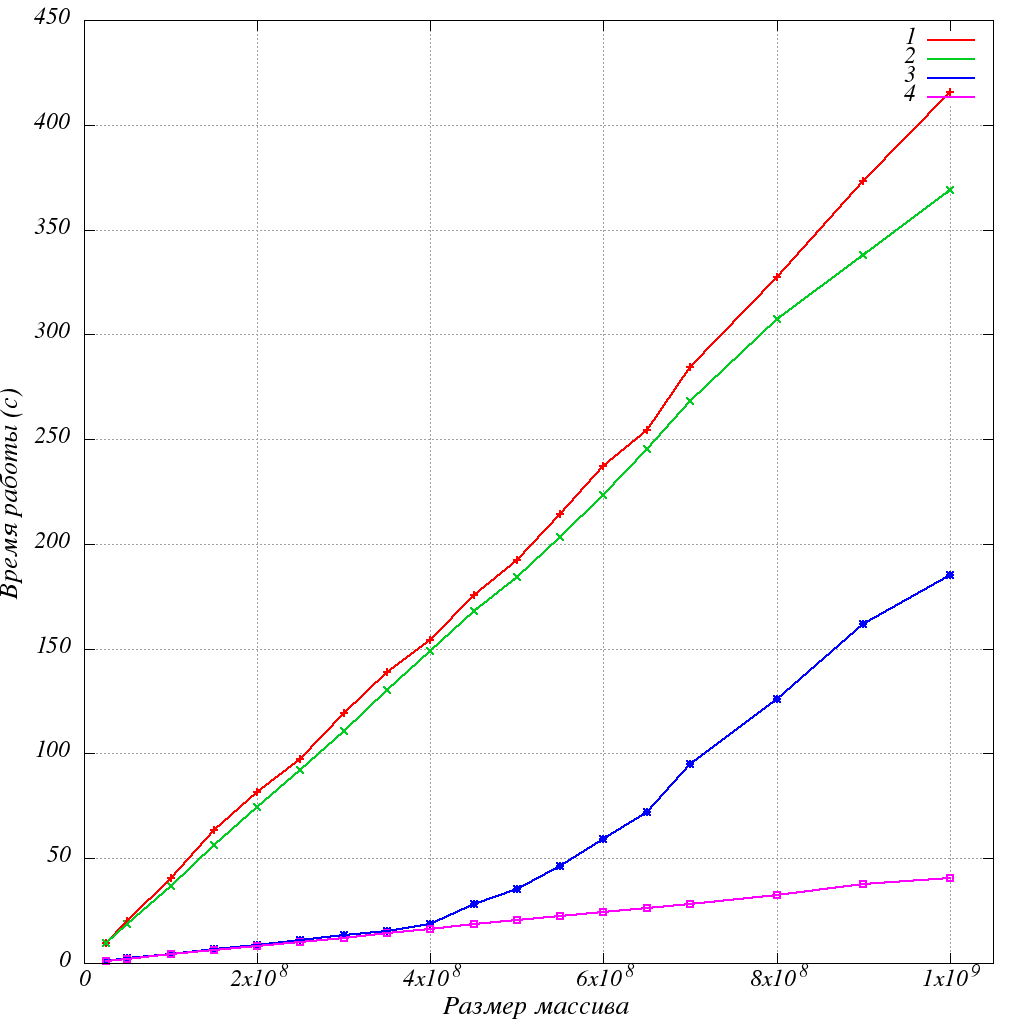
\includegraphics[width=1\linewidth]{./pics/graphics.png}}
\caption{
1 -- стандартная печать с записью на диск;
2 -- стандартная печать с записью в разделяемую память;
3 -- алгоритм параллельной печати с записью на диск;
4 -- алгоритм параллельной печати с записью в разделяемую память.} \label{grap}
\end{figure}

Сначала хочется заметить, что стандартная печать не сильно замедляется при записи в диск. 
Все время скорость работы диска была порядка 40--50 Mb/s.
Диск фактически не оказывает никакого существенного влияния на работу.

Из графиков также видно, что при записи в \textit{shared-memory} отношение времени работы стандартного алгоритма и ускоренного постоянно, так как оба графика -- прямые.
Это значит, что ускорение одинаково на всех данных.

Однако, такого нельзя сказать в случае записи на диск.
На графике в точке $4 \cdot 10^8$ (9.6 GB) происходит излом: начинает ощущаться влияние диска. Именно это мы и наблюдали в Тесте 1 -- ускорение немного упало при $5 \cdot 10^8$.
С этого момента печать начинает упираться в диск.
При запуске тестов было замечено, что скорость записи на диск временами достигает 800-900 Mb/s.
Из-за слишком больших файлов (так файл при размере массива $10^9$ достигает 24 GB) создается очередь из буферов на печать.
Потоки-обработчики обрабатывают буферы быстрее, чем производится сама печать.
Разница между третьим и четвертым графиком -- накладные расходы на работу диска.


%\newpage
\section{Заключение}
В результате написания курсовой работы была решена поставленная задача: 
реализована библиотека параллельной записи массивов вещественных чисел.

В ходе тестирования была проверена точность работы реализованного алгоритма, а также измерено ускорение в сравнении со стандартнйо функцией печати. 

Написанная на языке \textsf{С++} подпрограмма была внедрена в промышленный гидродинамический симулятор \textsf{tNavigator}.


%\newpage
\begin{thebibliography}{}

\bibitem{1} \textsc{Florian Loitsch}.
Printing Floating-Point Numbers Quickly and Accurately with Integers, 2004.
\bibitem{2} \textsc{Wojciech Mu\l a}.
SSE: conversion integers to decimal representation, 2011.


\end{thebibliography}


\end{document}
